\section{Opgave 5}

\begin{frame}{a) Produktionsmulighedsområdet}
\begin{itemize}
  \item Ugentlig produktion (hvis de udelukkende producerer 1 vare)
  \begin{itemize}
    \item Anders: $(F,K)_A = 6\cdot (2,1) = (12,6)$
    \item Helle: $(F,K)_H = 6 \cdot (1,2) = (6, 12)$
  \end{itemize}
\end{itemize}
\begin{figure}
\centering
    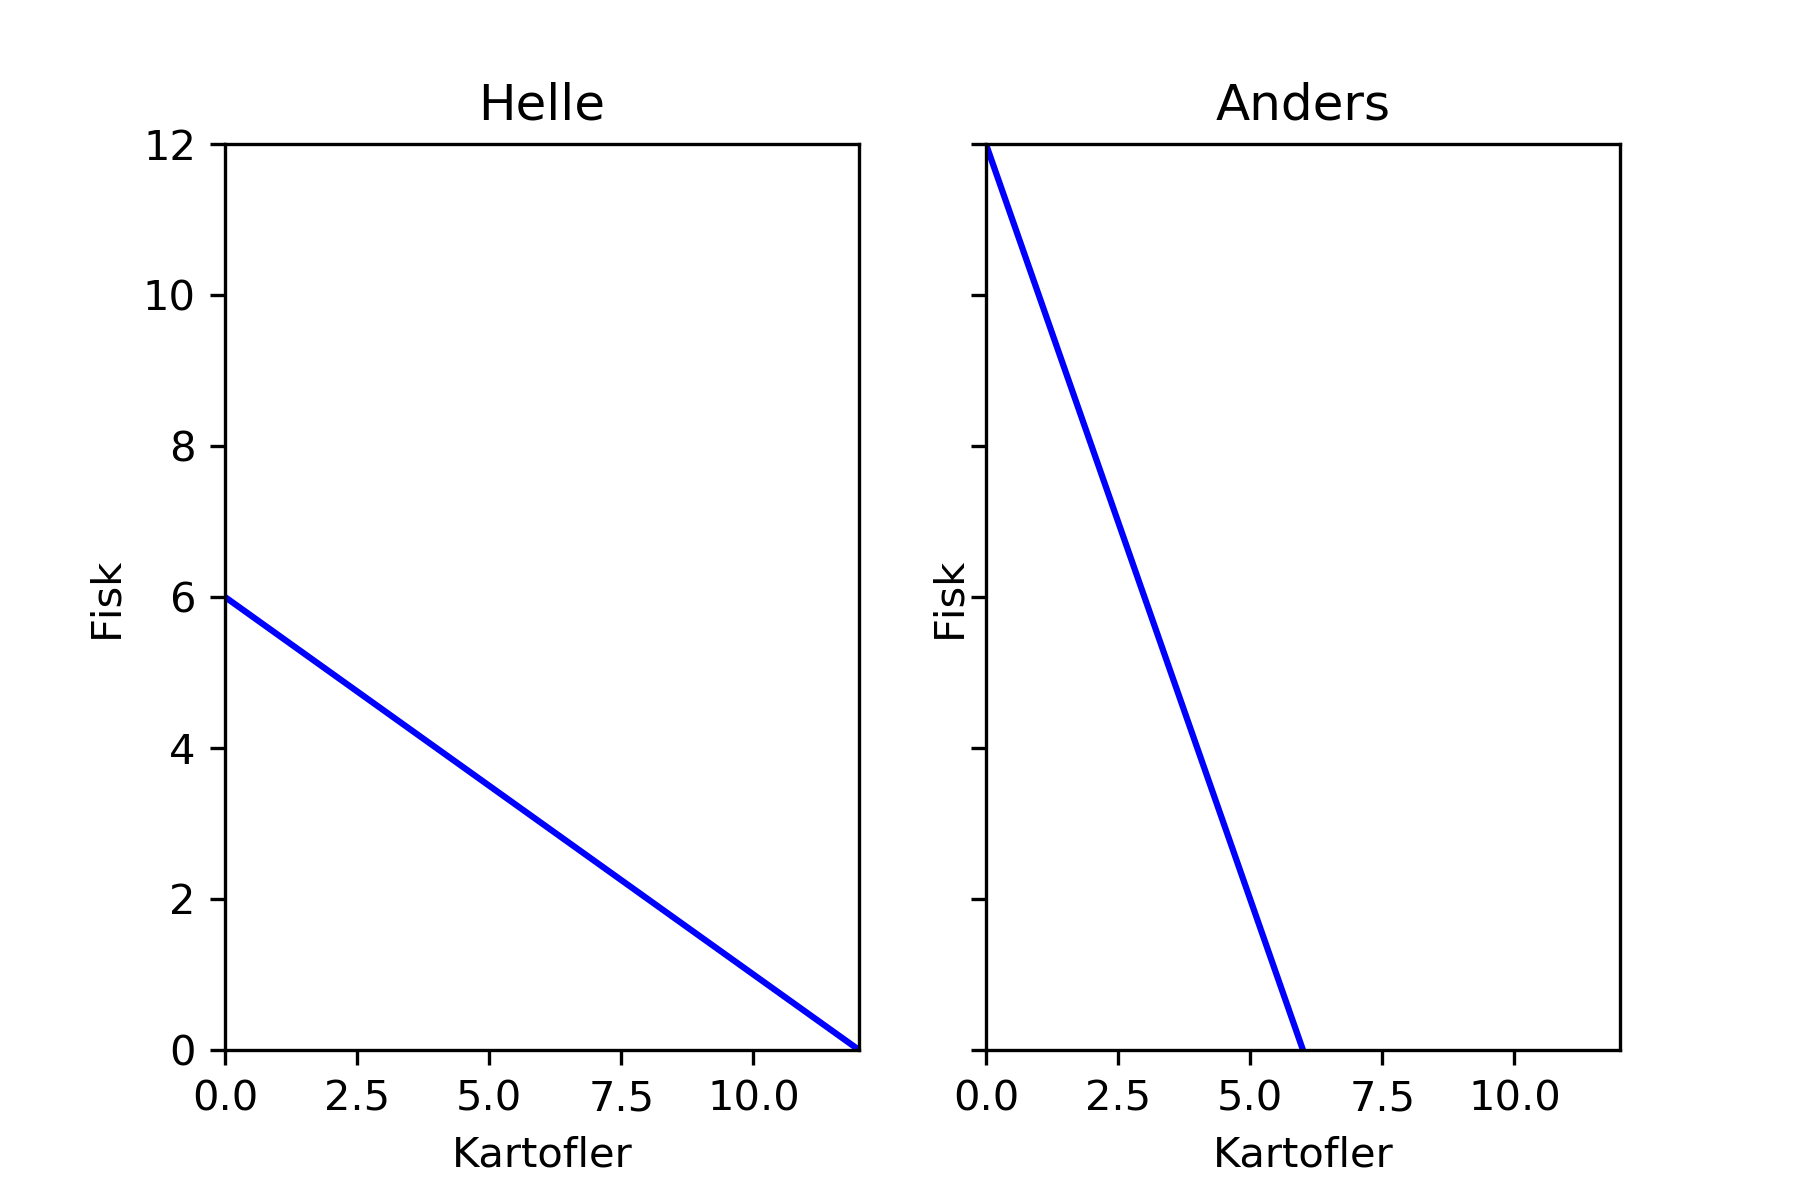
\includegraphics[width=0.6\textwidth]{img/comp2}
\end{figure}
Hvad er ligningerne for de to linjer?
\only<2>{\begin{itemize}
  \item Anders: $F_A(K_A) = 12 - 2K_A$
  \item Helle: $F_H(K_H) = 6 - \frac{1}{2}K_H$
\end{itemize}}
\end{frame}


\begin{frame}{b) Forbrug uden handel}
Husk at de begge kun vil forbruge lige dele fisk og kartofler, så for dem begge gælder at $F=K$.

\textbf{Anders:}
\begin{align*}
  F_A &= 12-2K_A \\
  & = 12 - 2F_A \\
  F^*_A &= 4
\end{align*}
Indsæt $F_A = 4$ i den oprindelige ligning
\begin{align*}
  4 &= 12 -2K_H \\
  K^*_H &= 4
\end{align*}
\textbf{Helle:}

Vi kunne gøre som for Anders, men fordi $F_H(K) = F_A^{-1}(K)$ og $F_A^*=K_A^*$ er løsningen $(F_H^*, F_K^*) = (4,4)$.
\end{frame}


\begin{frame}{c) Produktionsmulighedsområde og alternativomkostninger?}

\begin{itemize}
  \item \textbf{Hvad er sammenhængen mellem produktionsmulighedsområdet og alternativomkostningerne?}
  \begin{itemize}
    \item Hældningen på området er en alternativomkostning - \textit{"Hvis Helle øger produktionen af kartofler med 1kg, må hun sænke produktionen af fisk med $\frac{1}{2}$kg".}
  \end{itemize}
  \item \textbf{Hvem har de komparative fordele?}
  \begin{itemize}
    \item Kartofler: Helle. Hun skal kun sænke produktionen af fisk med 1/2 kg for at producere 1kg kartofler ekstra.
    \item Fisk: Anders. Hvorfor?
  \end{itemize}
\end{itemize}

\end{frame}


\begin{frame}{d) Påvirker handel situationen?}

Antag fuld specialisering - så producerer Anders 12kg fisk, og Helle 12kg kartofler. De vil kun forbruge i forholdet 1:1, så de kan bytte 6kg fisk for 6kg kartofler og forbruge $(F,K)=(6,6)$.

\end{frame}

\begin{frame}{d) Påvirker handel situationen?}
\begin{figure}
\centering
    \includegraphics<1>[width=0.9\textwidth]{img/comp2_analysis}
    \includegraphics<2>[width=0.9\textwidth]{img/comp2_analysis_arrow}
\end{figure}

\end{frame}


\begin{frame}{e) Ændring i Helles produktion}
Læg mærke til at ændringen øger helles produktion af både fisk og kartofler forholdsmæssigt lige meget. Derfor er der stadig komparative fordele.

De absolute fordele Anders havde i produktion af fisk er dog forsvundet. 
\end{frame}
